\section{GUI Components}\label{sprint3:gui}
During this sprint we also implemented the use of the shared GUI components, through the library \lstinline|giraf-components|.
We used two components; \lstinline|GButton| and \lstinline|GColorPicker|.
Additionally we used the standard background color, provided by the library.
The button and colorpicker components can be seen in \cref{sprint3:guicomponents:fig}.

\begin{figure}[h]
\begin{subfigure}{0.49\textwidth}
\centering
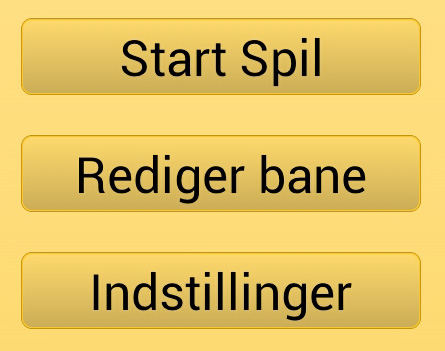
\includegraphics[width=0.49\textwidth]{sprint3/gbutton}
\caption{The \lstinline|GButton|s in Cars main Activity}
\label{sprint3:guicomponents:fig:gbutton}
\end{subfigure}
~
\begin{subfigure}{0.49\textwidth}
\centering
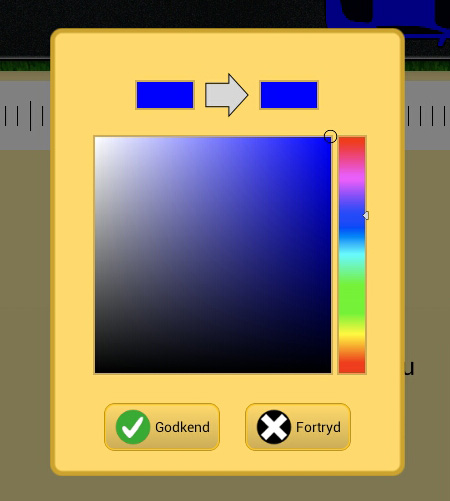
\includegraphics[width=0.49\textwidth]{sprint3/gcolorpicker}
\caption{\lstinline|GColorPicker| in Cars settings Activity}
\label{sprint3:guicomponents:fig:gcolorpicker}
\end{subfigure}

\caption{The graphics used in the game}
\label{sprint3:guicomponents:fig}
\end{figure}

\paragraph{Background color}
The main menu and setting activites were changed to use \lstinline|giraf-component|'s default background color, through the \lstinline|GetBackgroundColor()| method in the \lstinline|GComponent| class.

\paragraph{Buttons}
All menu-related buttons were changed to \lstinline|GButton|, which overrides the standard Android \lstinline|Button|.
No functionality is any different for the button, only layout.

\paragraph{Colorpicker}
The colorpicker was used for selecting car/garage colors, as mentioned in \cref{sprint3:settings}.
\lstinline|GComponent|'s \lstinline|GColorPicker| is an extension of \lstinline|GDialog|, which is an extension of Android's \lstinline|Dialog|.
The initial color of the dialog must be set by its \lstinline|SetCurrColor(int color)| method.
The new color, after choosing one in the dialog, is returned through the \lstinline|OnOkListener| interface, which provides the method \lstinline|OnOkClick(GColorPicker diag, int color)|.